
%-----------------------------------------------------
%
%    Contents
%
%-----------------------------------------------------


\sectionfix
\section{Related Work}
\label{sec:relatedwork}
The HCI field of exploring the body as an input surface for possible interactions has been widely researched throughout the past years. Rapidly growing topics include the use of wearable systems, various sensing techniques and multi-touch input.\newpara
In this chapter, related work is discussed in the context of gestural 3D modeling, skin-based fabrication, and fabrication-aware design. The key ideas and limitations of the respective approaches are summarized at the end.
\subsection{On-Body Interaction}
\label{subsec:body}
The body is the most confidential and familiar interactive system to the human race.
The skeleton of a human arm affords a natural degree of freedom ( DOF ) offering a wide range of application possibilities \cite{Harrison:2012:OIA:2148131.2148148}. Additionally, interactions with the arm can always be accessible without the need for visual awareness to the target device \cite{Gustafson:2013:UPI:2470654.2466114}.
This always-available aspect combined with the unique context of using our body as a platform for access to communication and computation have proven to be a wide area of exploration \cite{Harrison:2011:OWM:2047196.2047255, Harrison:2010:SAB:1753326.1753394, Nittala:2018:MST:3173574.3173607, Dezfuli:2012:PIP:2325616.2325623, Gustafson:2011:IPL:2047196.2047233} and results received considerable attention in the HCI community.\newpara
Several papers focus their investigation on technical approaches for on-skin devices with touch-based capabilities. The research scope includes the use of capacitive sensing \cite{Kao:2016:DRP:2971763.2971777,Weigel:2015:IFS:2702123.2702391, Kao:2015:NFI:2702123.2702572}, on-body projection \cite{Harrison:2011:OWM:2047196.2047255, Harrison:2010:SAB:1753326.1753394, Xiao:2018:LOP:3173574.3173669}, ultrasound transmission \cite{Mujibiya:2013:STO:2512349.2512821}, magnetic \cite{Chan:2013:FPS:2501988.2502016} and electro-wave propagation \cite{Zhang:2016:SUB:2858036.2858082}. A particular interesting area is the use of optical devices to establish realistic touchable surfaces \cite{Harrison:2011:OWM:2047196.2047255}.\label{subsec:camera}
Hereby, researchers have advanced to augment physical context with the virtual modeling setting \cite{Leithinger:2011:DGI:2047196.2047268, Follmer:2012:KDR:2207676.2208403, Follmer:2010:CRP:1866218.1866230}. This trend aids novices to gain a more familiar feeling and hence incorporate a better understanding of the digital environment into their design \cite{Gannon:2015:TSA:2702123.2702581}.
A specific work by Andre D. Wilson \cite{Wilson:2010:UDC:1936652.1936665} investigates the application of depth-sensing cameras to identify touch input on a tabletop. Results illustrate that touch sensing is even possible on complex surfaces - such as concave or twisted regions - and allow a variety of unique interactions e.g.\;determine different hover states by measuring the distance between finger and target object.
One step ahead, Dezfuli et al.\cite{Dezfuli:2012:PIP:2325616.2325623}\;study in their paper ``\,PalmRC: Imaginary palm-based Remote Control for Eyes-free Television Interaction\," the possibilities of leveraging the palm as an interactive surface for TV remote control. They use an RGB-D camera - which is anchored on top of the television - to track gestural movements and identify distinctive tasks. A considerable benefit is that no calibration is required before sensing a palm of a different person. Each user presented with the device was able to immediately interact with the tool. However, both methods are restricted in their specific location area i.e.\;it was not possible to communicate with the system out of the cameras perception range. Our intention is to utilize the strength of the camera set-up to design a personalized sensor which the user can carry on the body. This provides the freedom of maximum mobility.
\newpara
Another important contribution, ``\,ExoSkin: On-Body Fabrication\," by Gannon et al.\;\cite{Gannon:2016:EOF:2858036.2858576} uses a custom built extruder to directly print on a drawn path which is projected onto the arm. Alternatively, the designed geometry can be exported and traditionally processed with a 3D printer and appropriate materials. However, the system uses a motion capture system which is considered costly to maintain. Authors stated that other tracking technologies should be considered such as the depth-sensing camera Kinect \cite{Zhang:2012:MKS:2225053.2225203}. Initial experimentation with the device resulted in a lack of accuracy. We anchor on this idea by utilizing the second generation version of Kinect which has a more reliable data stream than its predecessor \cite{wasenmuller2016comparison}.\\




Important in this context is the work ``\,Multi-Touch Skin: A Thin and Flexible Multi-Touch Sensor for On-Skin Input\," by Nittala et al.\,\cite{Nittala:2018:MST:3173574.3173607}. The group presents a novel fabrication approach for printing thin-layered mutual-capacitance-based touch sensors and is the first to achieve a high-resolution multi-touch capability (see \textbf{\autoref{fig_multitouch}}). Their fabricated overlay is able to withstand extreme deformations which can occur on local maxima of curvature, such as the wrists or similar joints. Furthermore, their study outcome scores in robustness, functionality and scalability and flags them as desirable features for future projects. However, authors stated that creating an input surface needs to consider the unique body properties such as the size.
Hence, a crucial requirement was the development of an interactive and intuitive design tool that can generate sensor layouts given any arbitrary 2D shape. The group stated that a limitation of the tool was the lack of a body measuring process and that subsequent work could include a scanning task into the existing pipeline. Our approach is tailored to this demand and provides a computer vision method to improve iterative design for on-skin devices.
Furthermore, Scansify creates a flatten 2D overlay that can be further processed to a thin-layered sensor as described above. Hence, our tool can be directly included as a preprocessing step for most projects.
\begin{figure}[H]
    \captionit
    \centering
    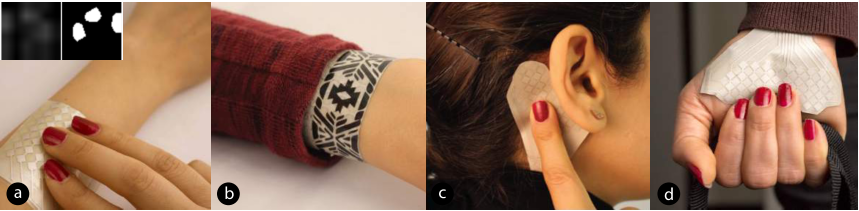
\includegraphics[scale=0.65]{pictures/multitouch.png}
    \caption{Multi-touch skin. Figure acquired from \cite{Nittala:2018:MST:3173574.3173607} \\
    a) multi-touch input on the forearm for remote interaction;\\
    b) aesthetic bracelet with multi-touch capabilities;\\
    c) input surface close to the ear for audio context;
    d) sensors for busy hands}
    \label{fig_multitouch}
\end{figure}
Lo et al.\;\cite{Lo:2016:SDC:2901790.2901885} introduce in
``\,Skintillates: Designing and Creating Epidermal Interactions\," a wearable technology using conductive silver ink on tattoo paper. The thin-layered sensors naturally wrap around the user's skin which, combined with the decorative design, facilitate an expressive and personal display. Application examples include capacitive buttons for mobile device control, body position detection and a light-emitting diode ( LED ) display that reacts to music. One of its fabrication challenges was to provide users, that do not have the technical knowledge for producing such devices, a sophisticated approach for flexible visual and electrical design. Therefore, the production cost of Skintillates was greatly reduced by integrating commonly available materials and easy-to-afford equipment. Still, the time consumption of building a specific device does highly vary with the design process of a tattoo pattern. The unique properties of a user's body make manually measuring the size of an arm a stagnant process. By importing our approach into their existing fabrication pipeline, it would enable a more flexible and rapid prototyping process for creating any personalized shape due to its capabilities on iterative design (see \textbf{\hyperref[item:functionality]{Chapter 1.1}})
. 
\newpara 
Recently, skin-friendly materials have been explored to replace the vastly expensive equipment to produce sensors. A successor to the approach of Skintilattes is ``\,DuoSkin: Rapidly Prototyping On-Skin User Interfaces Using Skin-Friendly Materials\," by Kao et al \cite{Kao:2016:DRP:2971763.2971777}. The group aims to make a durable on-skin circuitry available to non-experts in the HCI community by utilizing commodity materials. The device is able to sense touch input, to display an output and communicate wirelessly with other machines. Results from the user study show that the fabrication process was perceived ``\,fun and enjoyable\,". Furthermore, the ability to customize the devices with one's own design made it more intimate. Though, the design process uses paper stencils which limits the users in their customization experience. We share the same vision of providing users access to produce sensors without the demanding technical background. Furthermore, we believe that our tool can facilitate a faster and more individualistic approach to determine location and size of printed user interfaces. Scansify enables the users to draw any shape they desire and offers a flexible environment that encourages iterative rapid design.

\subsection{Design Tools in HCI for Fabrications}
The scientific contributions previously mentioned in \textbf{\autoref{subsec:body}} and \textbf{\autoref{subsec:camera}} have shown the demand for computational means to improve design iterations and sensor overlays for on-body interaction. Therefore, researchers have included external  graphics editor into their workflow e.g. Adobe Illustrator \cite{Kao:2016:DRP:2971763.2971777, Lo:2016:SDC:2901790.2901885}. However, the tools often lack flexibility and cannot be easily extendable in their own functionality. Hence, it is important to develop internal systems that are tailored specifically to personalized sensor modeling.\newpara
A novel approach is to engage the non-technical audience in advanced modeling with sketch-based 2D drawings \cite{Johnson:2012:SMS:2212776.2212390, Saul:2010:SAC:1935701.1935717}. One such system even incorporates the user to design and fabricate on the material itself \cite{Willis:2010:IFN:1935701.1935716, }. Based on a similar idea, ``\,Tactum: A Skin-Centric Approach to Digital Design and Fabrication\," by Gannon et al. \cite{Gannon:2015:TSA:2702123.2702581}\;presents a system to directly use the skin as the design interface. Tactum allows non-experts to intuitively create precise forms on top of the human body by capturing different gestures e.g.\;touch, grab, drag and rub. The implementation relies on a single depth camera that senses the input on the body. Additionally, a monitor is mounted on the desk to visualize a 3D representation of the arm and the drawn artwork on it (see \textbf{\autoref{fig:tactum_sub1}}). Results reveal that both experts and non-experts were enthusiastic about the system and further research could stabilize the feasibility of the project. The overly simplified representation of the arm was considered too coarse and was a highlighted limitation (see \textbf{\autoref{fig:tacum_sub2}}). It was suggested to portray the geometry of the arm and its texture more precisely to convey a more steady bridge between interaction and manipulation. Our work aims to investigate this idea further by digitally reconstructing the finer details of a human body through a depth stream.
\begin{figure}[H]
\centering
\captionit
\begin{subfigure}{.5\textwidth}
  \centering
  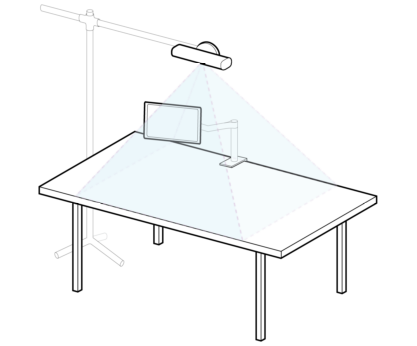
\includegraphics[width=.6\linewidth]{pictures/tactum_1}
  \caption{An illustrative drawing of the setup: The arm would be scanned on the desk}
  \label{fig:tactum_sub1}
\end{subfigure}%
\begin{subfigure}{.5\textwidth}
  \centering
  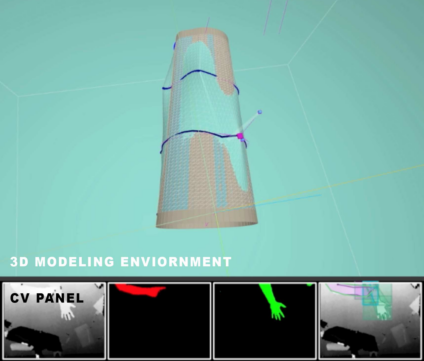
\includegraphics[width=.6\linewidth]{pictures/tactum_2}
  \caption{The design environment:\\3D model is live updated}
  \label{fig:tacum_sub2}
\end{subfigure}
\caption{Tactum. Figure acquired from \cite{Gannon:2015:TSA:2702123.2702581}}
\label{fig:tactum}
\end{figure}
\subsection{Summary}
This chapter presented an overview on the current vision and limitations of on-body interaction in the context of sensor design. In the past years, several researchers have explored the possibilities of sensing techniques and sensor capabilities. The wide range of investigation can include using different materials \cite{Lo:2016:SDC:2901790.2901885}, external tools \cite{Gannon:2016:EOF:2858036.2858576} or exploring different interaction possibilities \cite{Harrison:2012:OIA:2148131.2148148}. Still, these works often suffer from inprecise arm geometry acquisition \cite{ Gannon:2015:TSA:2702123.2702581}, lack of customization capability \cite{Kao:2016:DRP:2971763.2971777} or inflexibility from third-party drawing tools \cite{Kao:2016:DRP:2971763.2971777, Lo:2016:SDC:2901790.2901885}. Hence, an upcoming challenge and philosophy is to introduce intuitive fabrication methods that assists the user in building their own customized sensors. These works - including ours - depict an initial investigation on skin-centric design approaches. In the next chapter, ideas and findings from this scientific research are used to facilitate design recommendations for our tool and to overcome the prior mentioned limitations.

\newpage
\pagebreak